Интерфейс предполагает ввод всех необходимых параметров модели. Моделирование происходит до тех пор, пока не будет обработано 1\,000 сообщений. 

Также предоставляется возможность указания в процентах объема сообщений, которые возвращаются обратно в очередь.

На рисунках \ref{fig1:image} -- \ref{fig5:image} демонстрируются результаты работы.

\begin{figure}[h!]
	\begin{center}
		{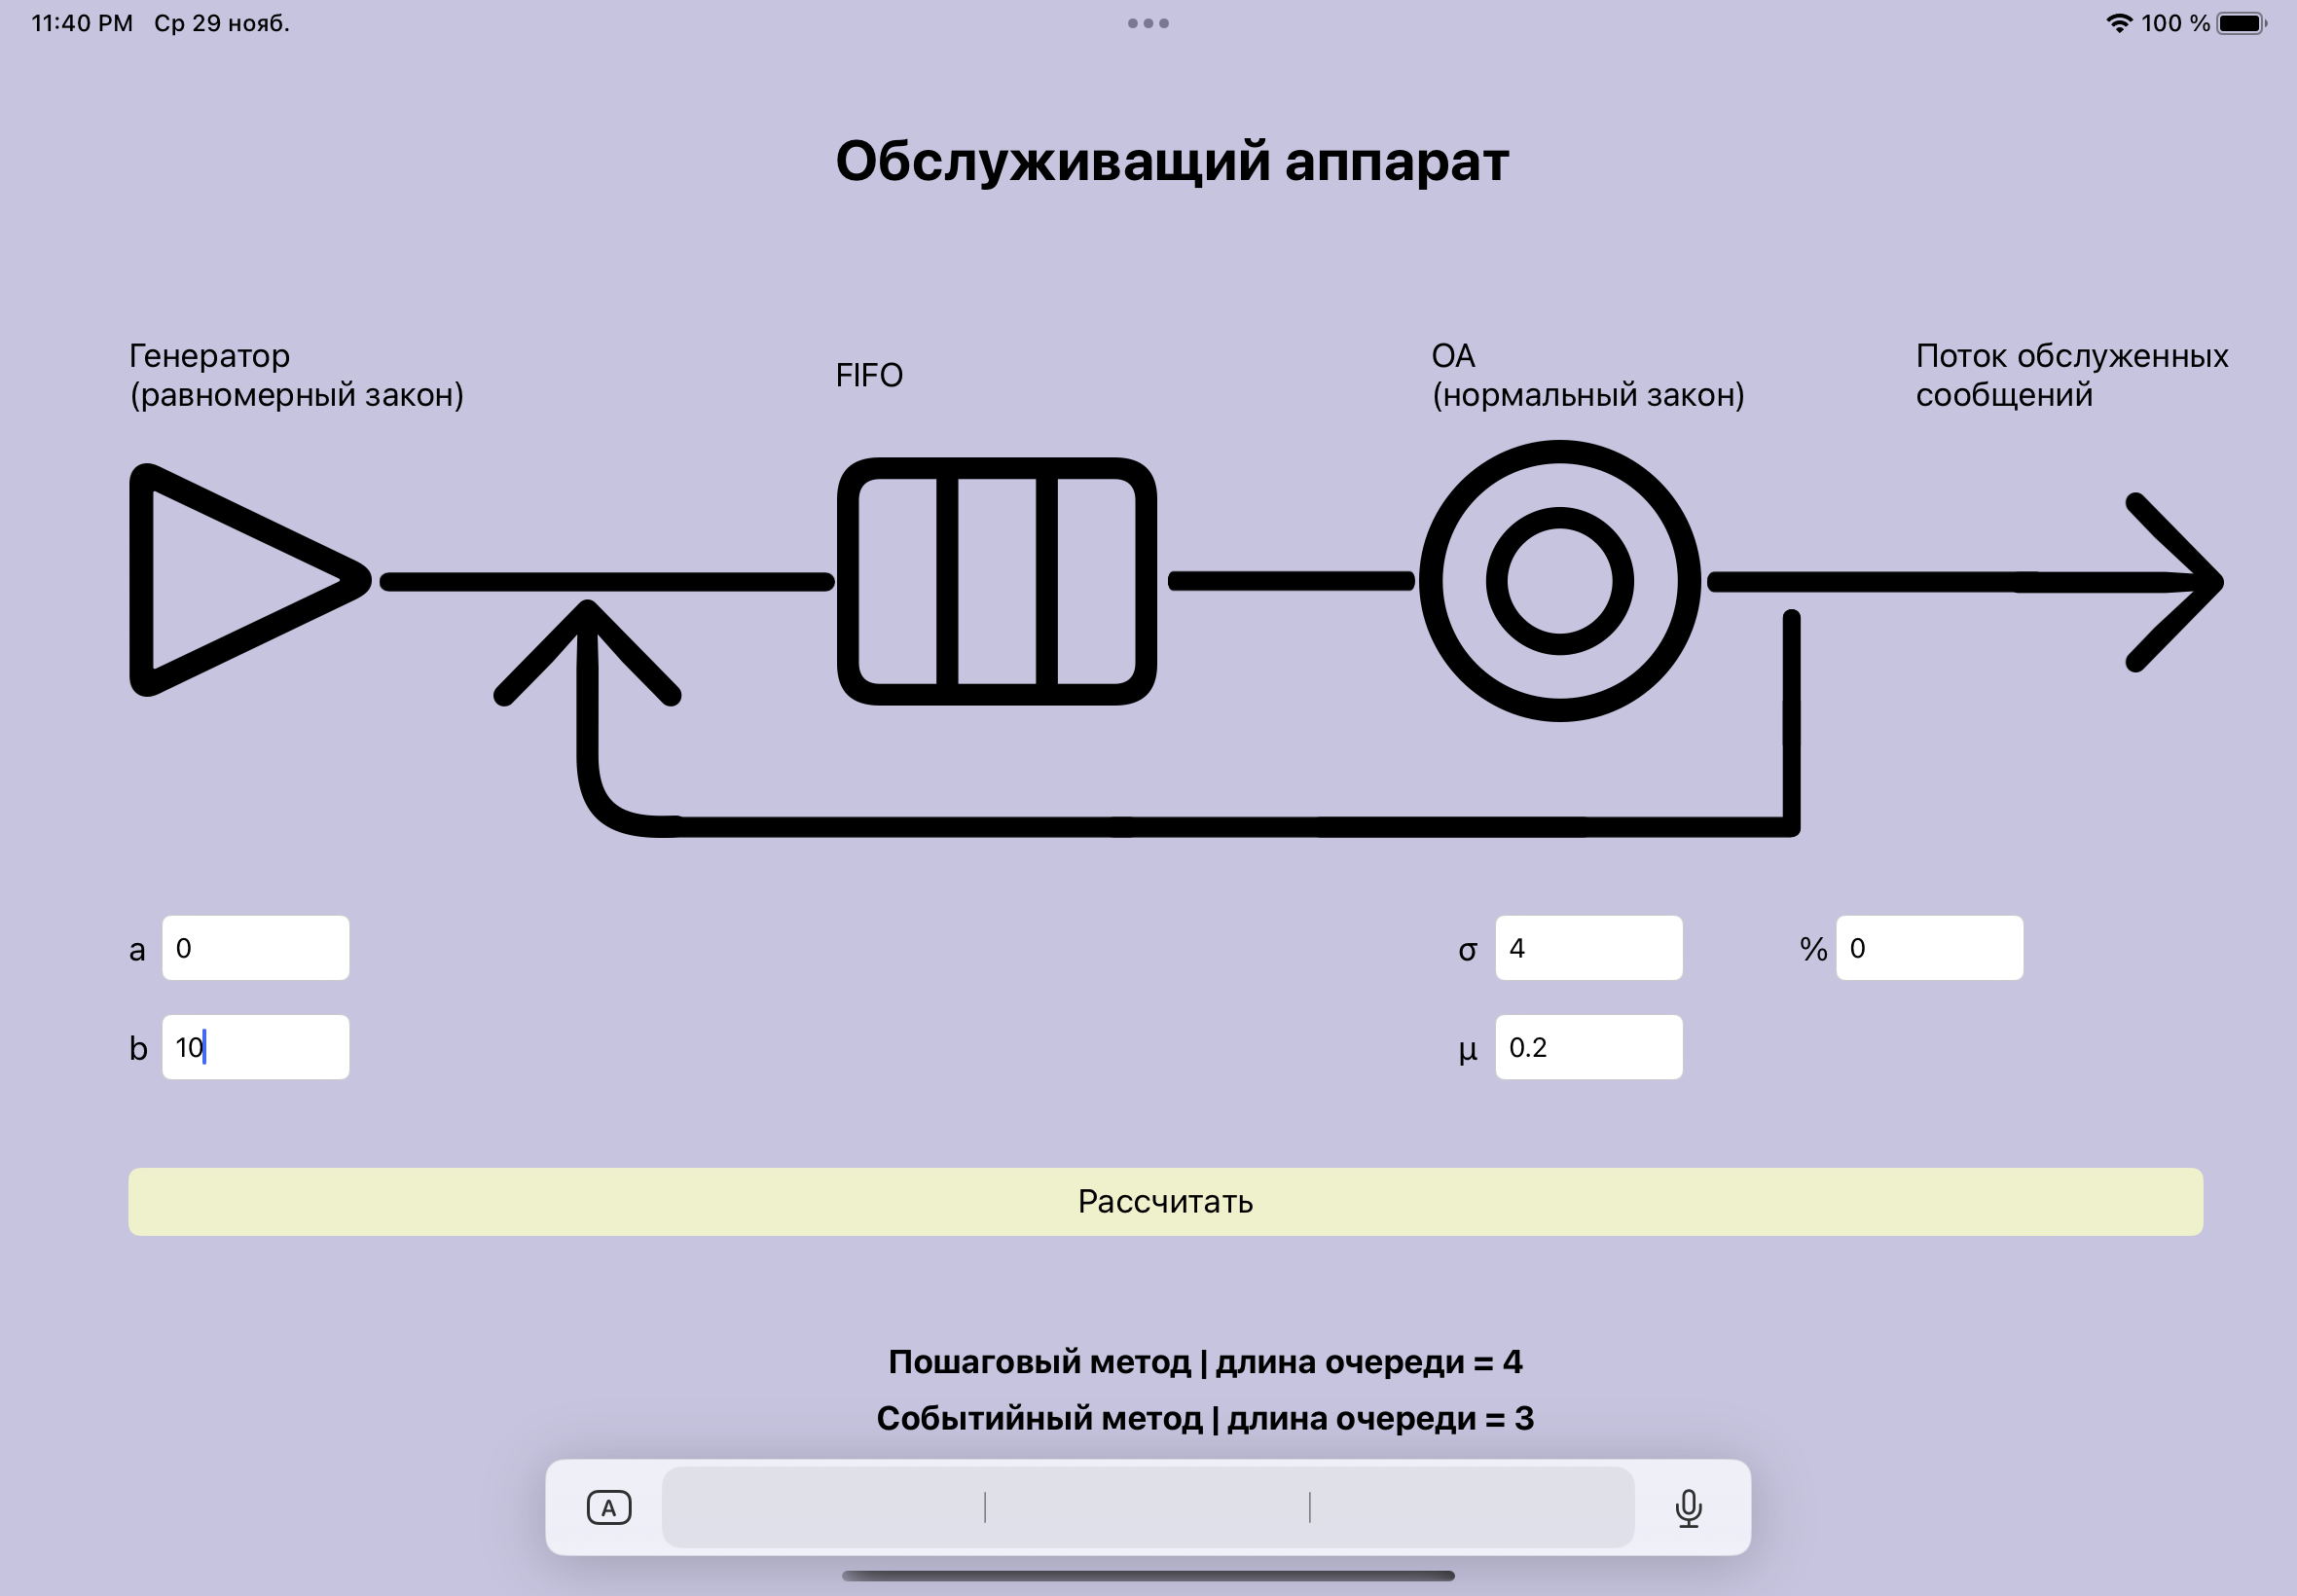
\includegraphics[scale = 0.15]{img/ex1.png}}
		\caption{Пример 1. Генератор и обслуживающий автомат работают с примерно одинаковой производительностью}
		\label{fig1:image}
	\end{center}
\end{figure}

\begin{figure}[h!]
	\begin{center}
		{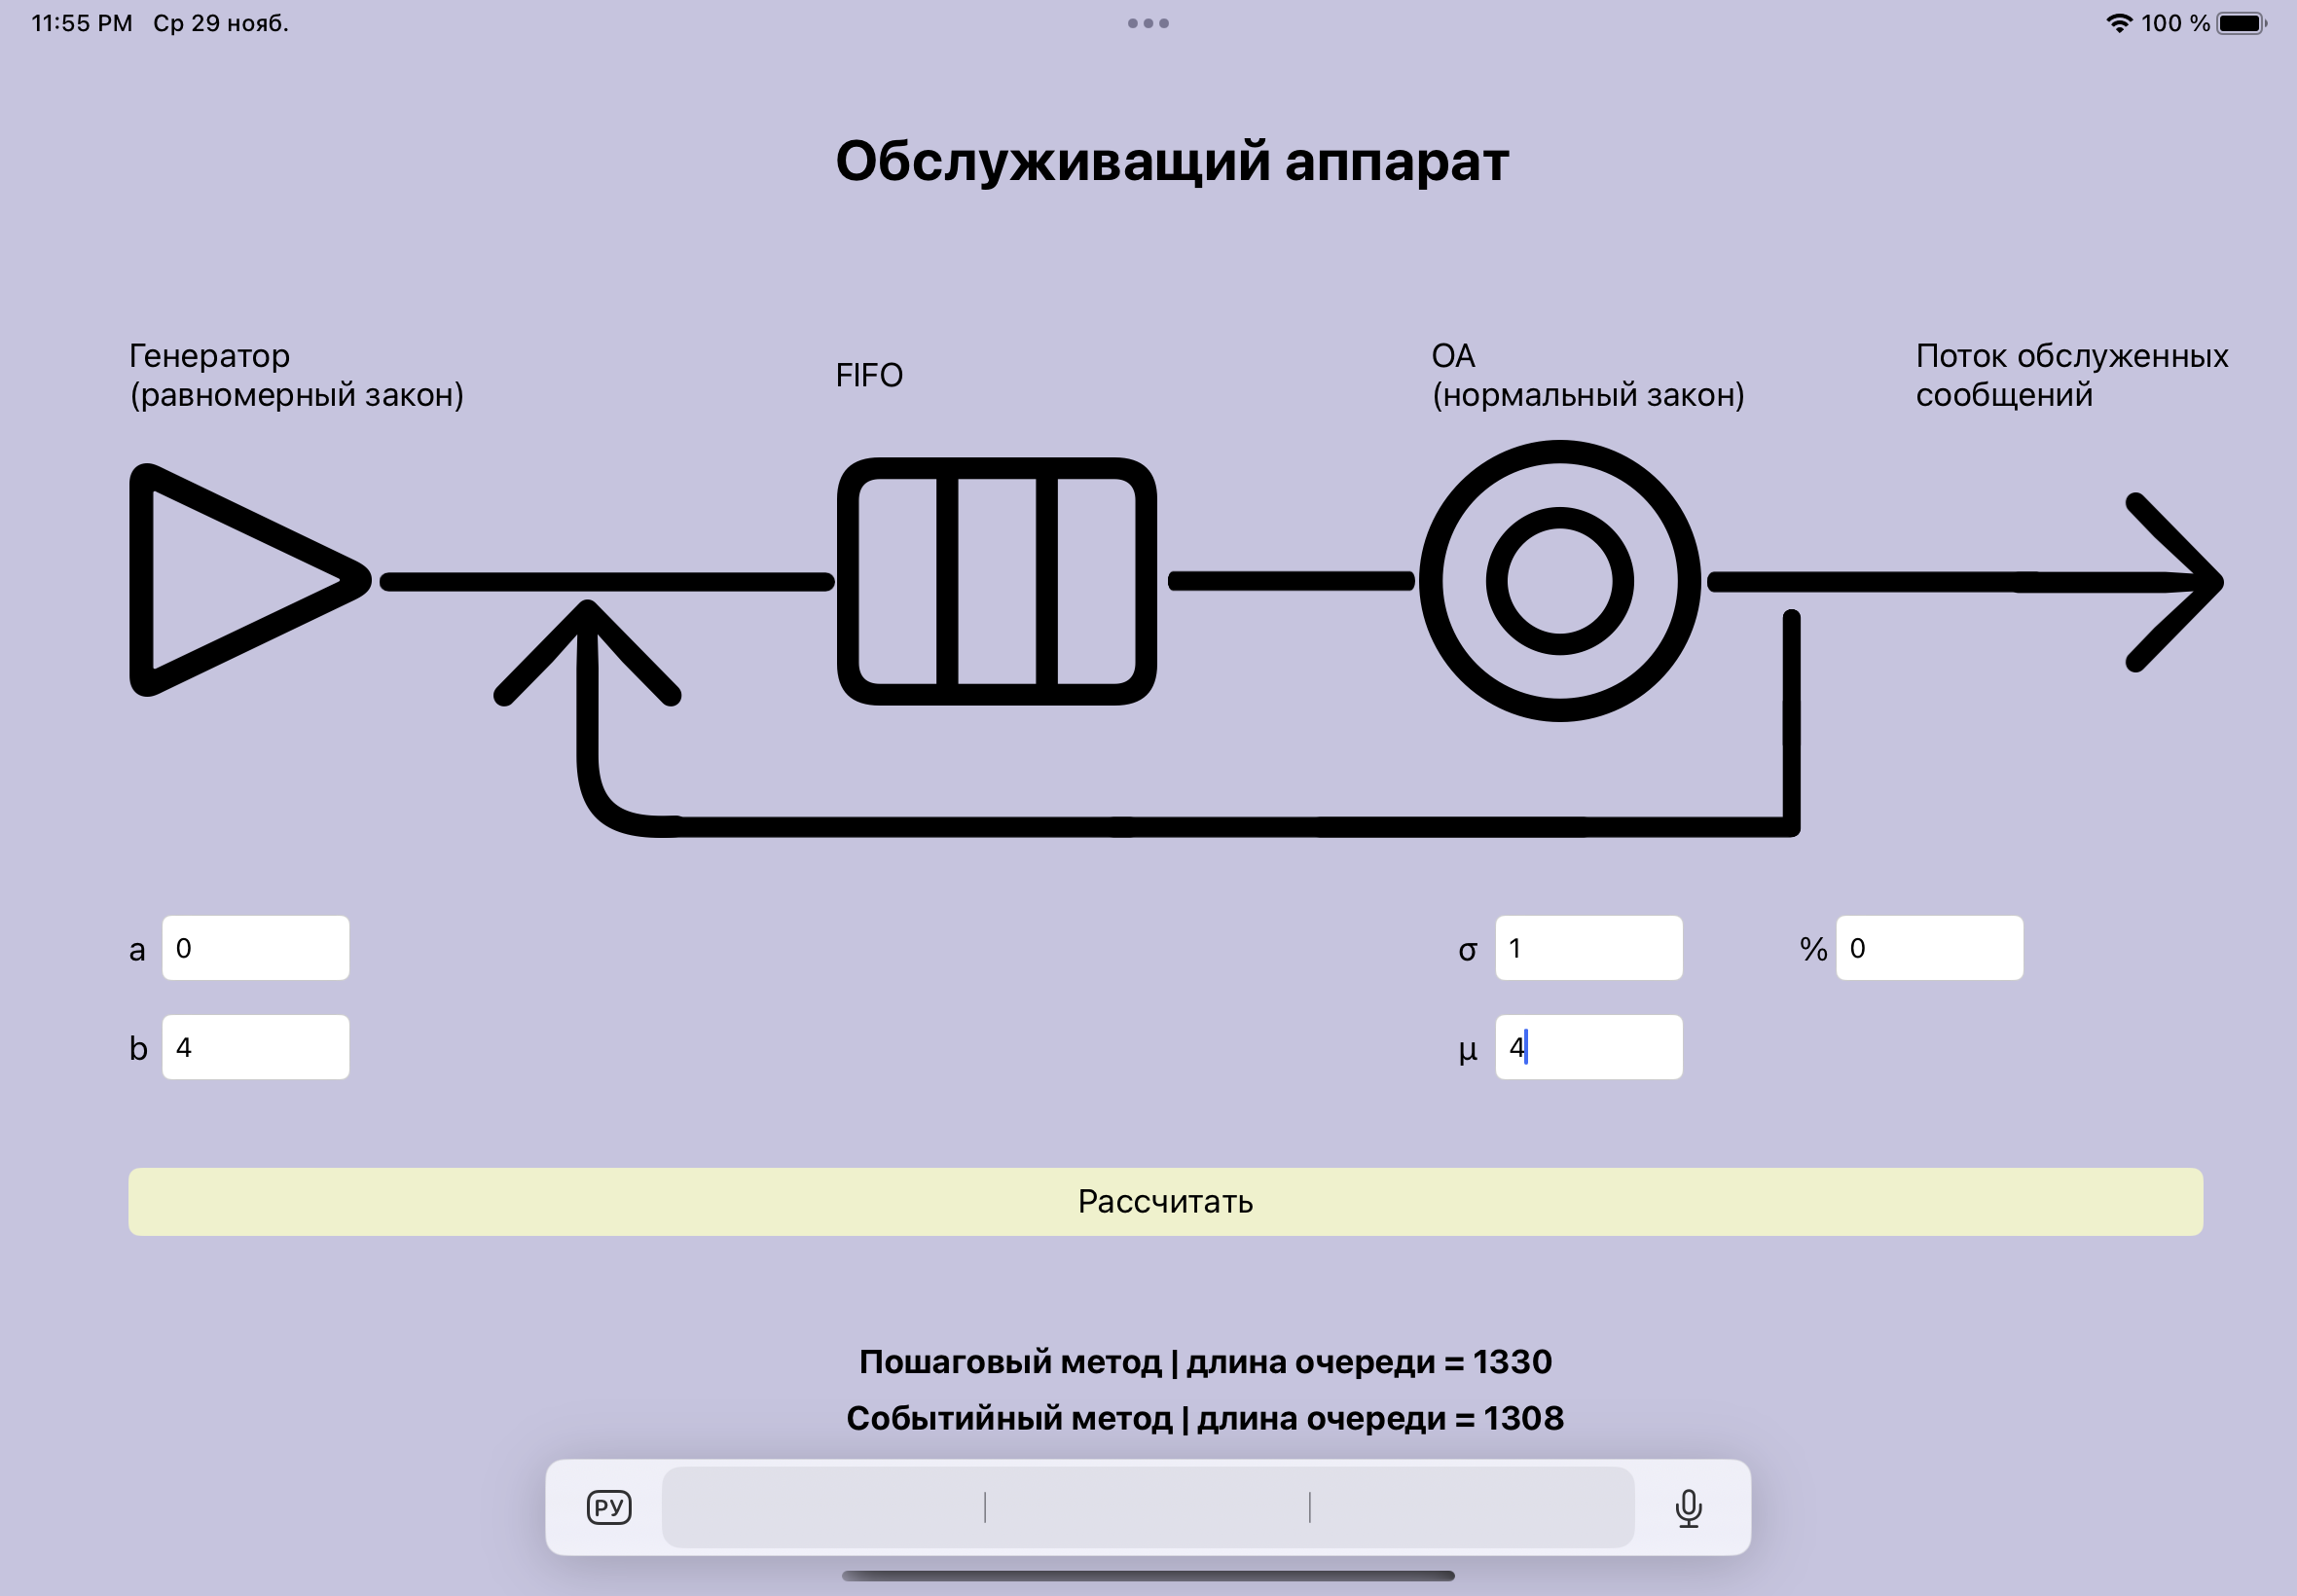
\includegraphics[scale = 0.15]{img/ex2.png}}
		\caption{Пример 2. Генератор создает сообщения интенсивнее, чем их обрабатывает автомат (при таких параметрах возникает переполнение)}
		\label{fig2:image}
	\end{center}
\end{figure}
\newpage

\begin{figure}[h!]
	\begin{center}
		{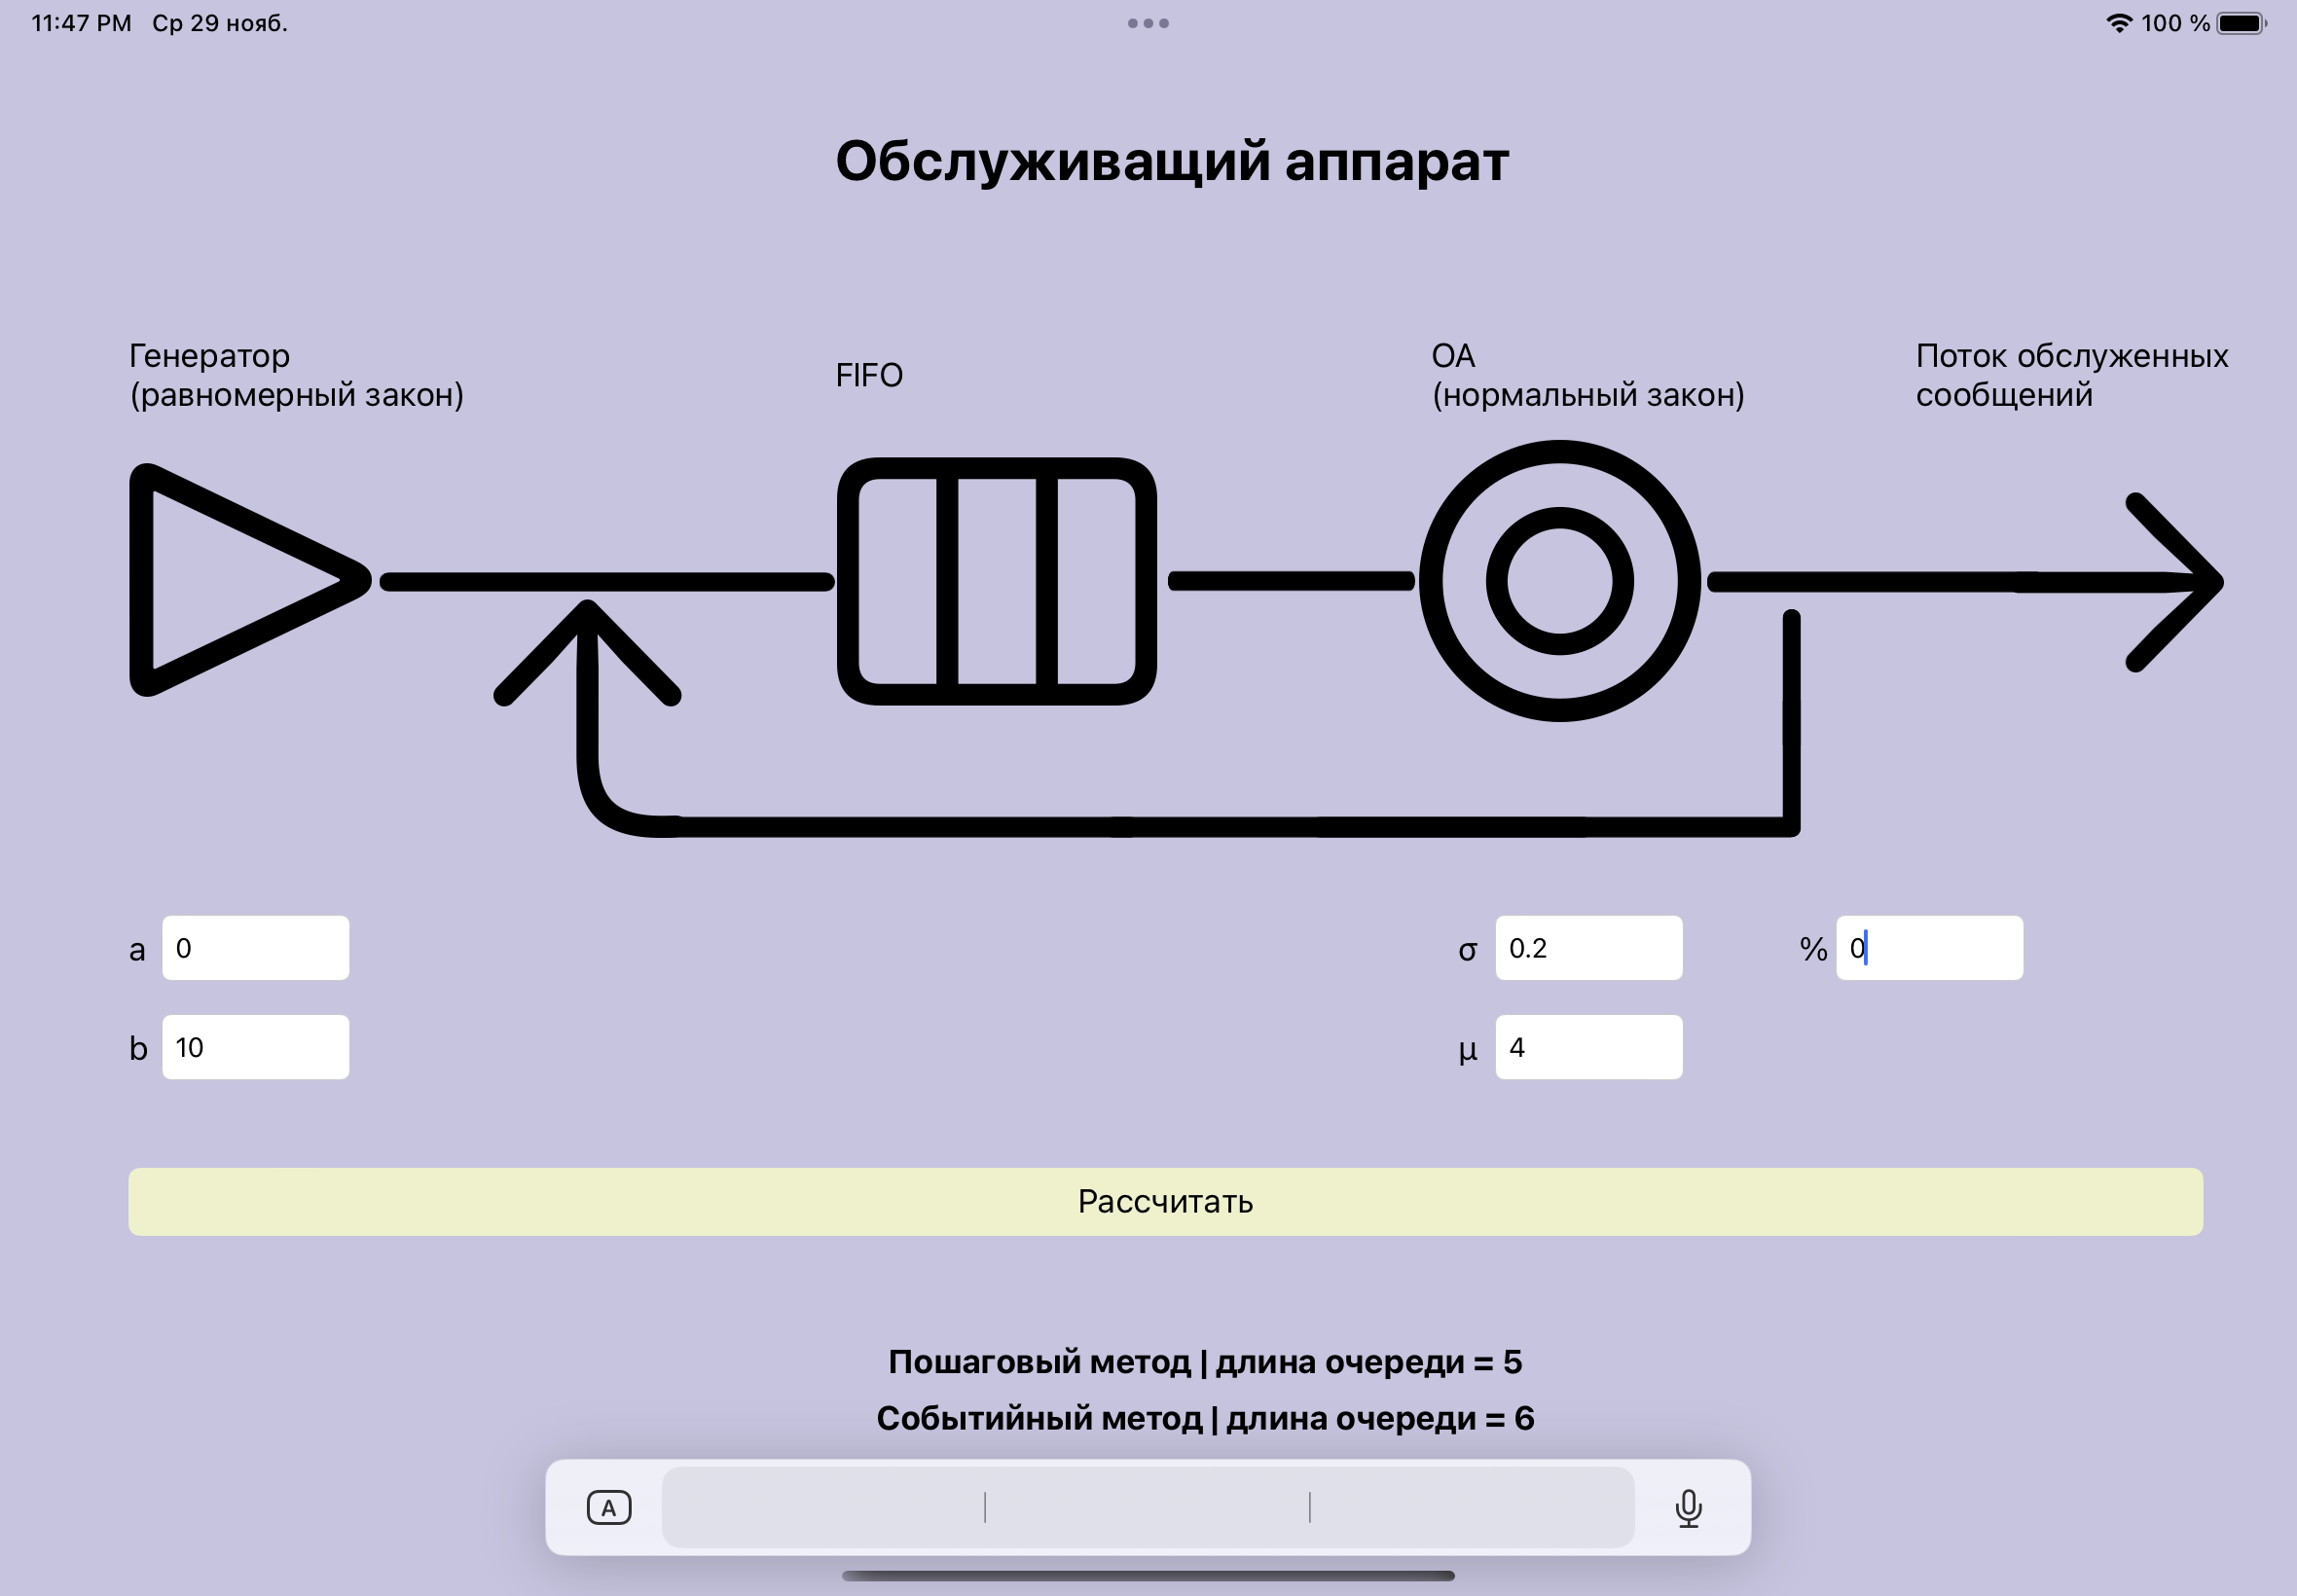
\includegraphics[scale = 0.15]{img/ex3.png}}
		\caption{Пример 3. Автомат обрабатывает сообщения интенсивнее, чем их создаёт генератор}
		\label{fig3:image}
	\end{center}
\end{figure}
\newpage

\begin{figure}[h!]
	\begin{center}
		{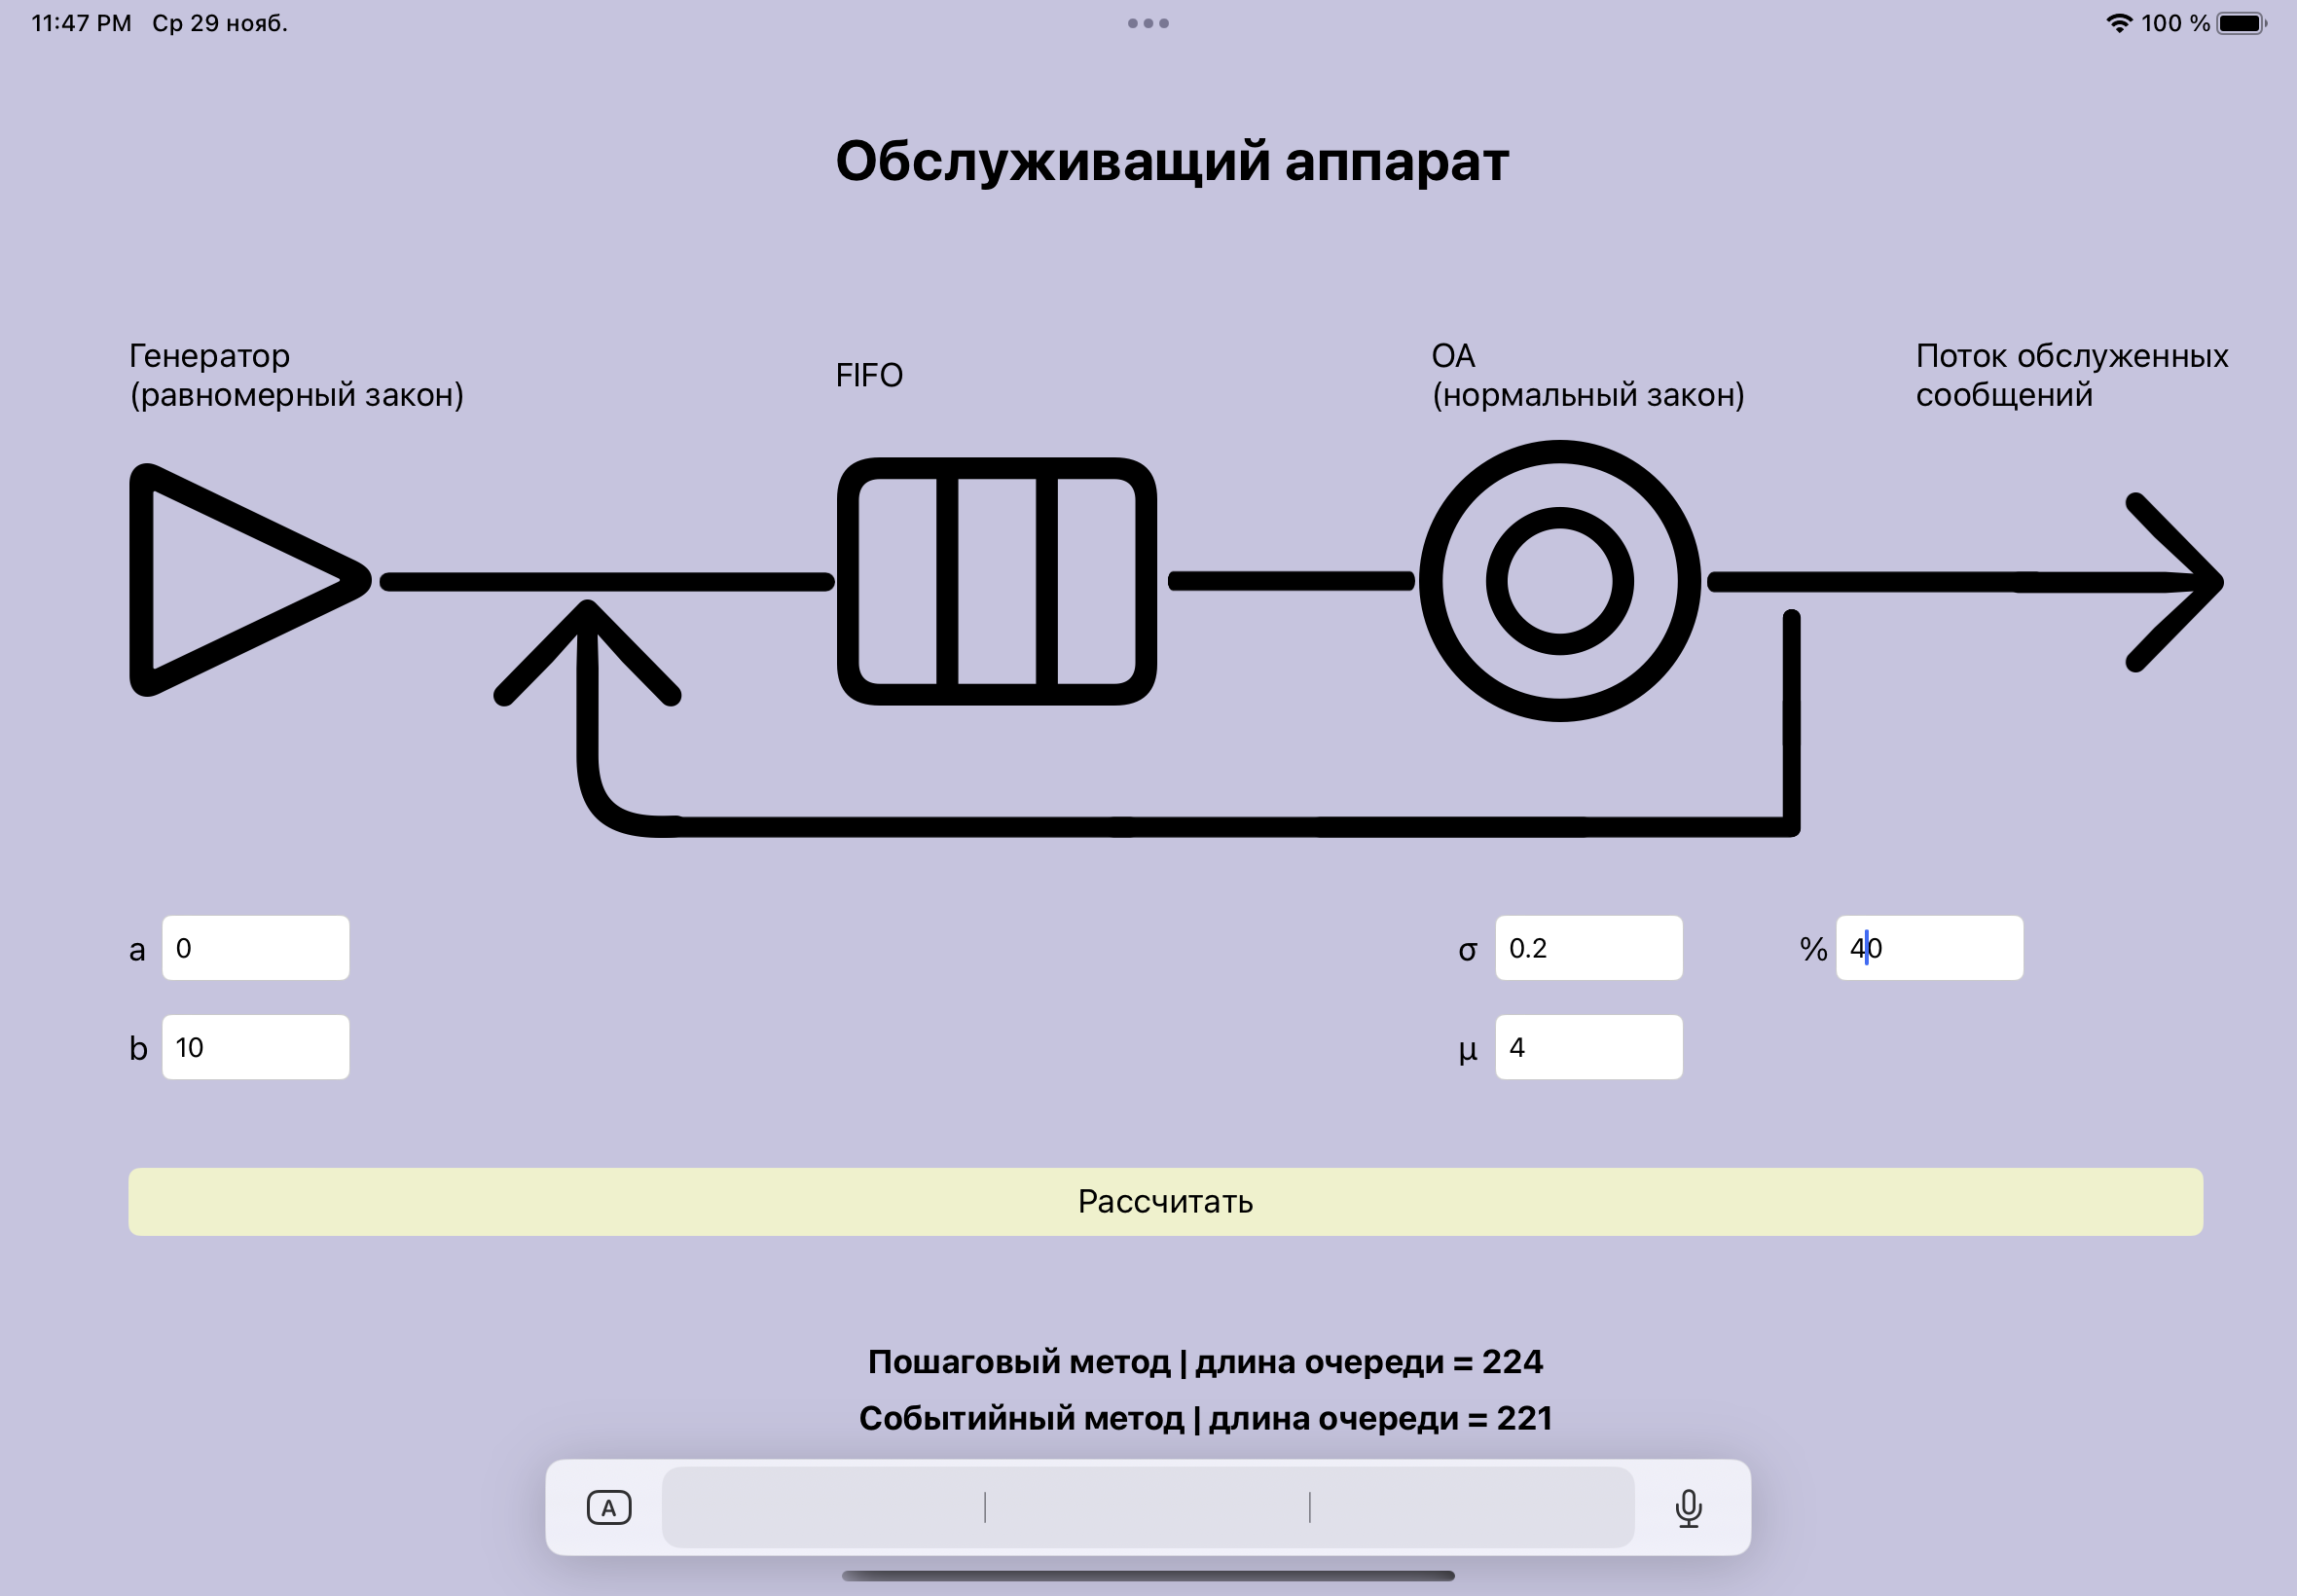
\includegraphics[scale = 0.15]{img/ex4.png}}
		\caption{Пример 4. Параметры такие же, как в примере 3, но есть процент возврата -- 40\%}
		\label{fig4:image}
	\end{center}
\end{figure}

\begin{figure}[h!]
	\begin{center}
		{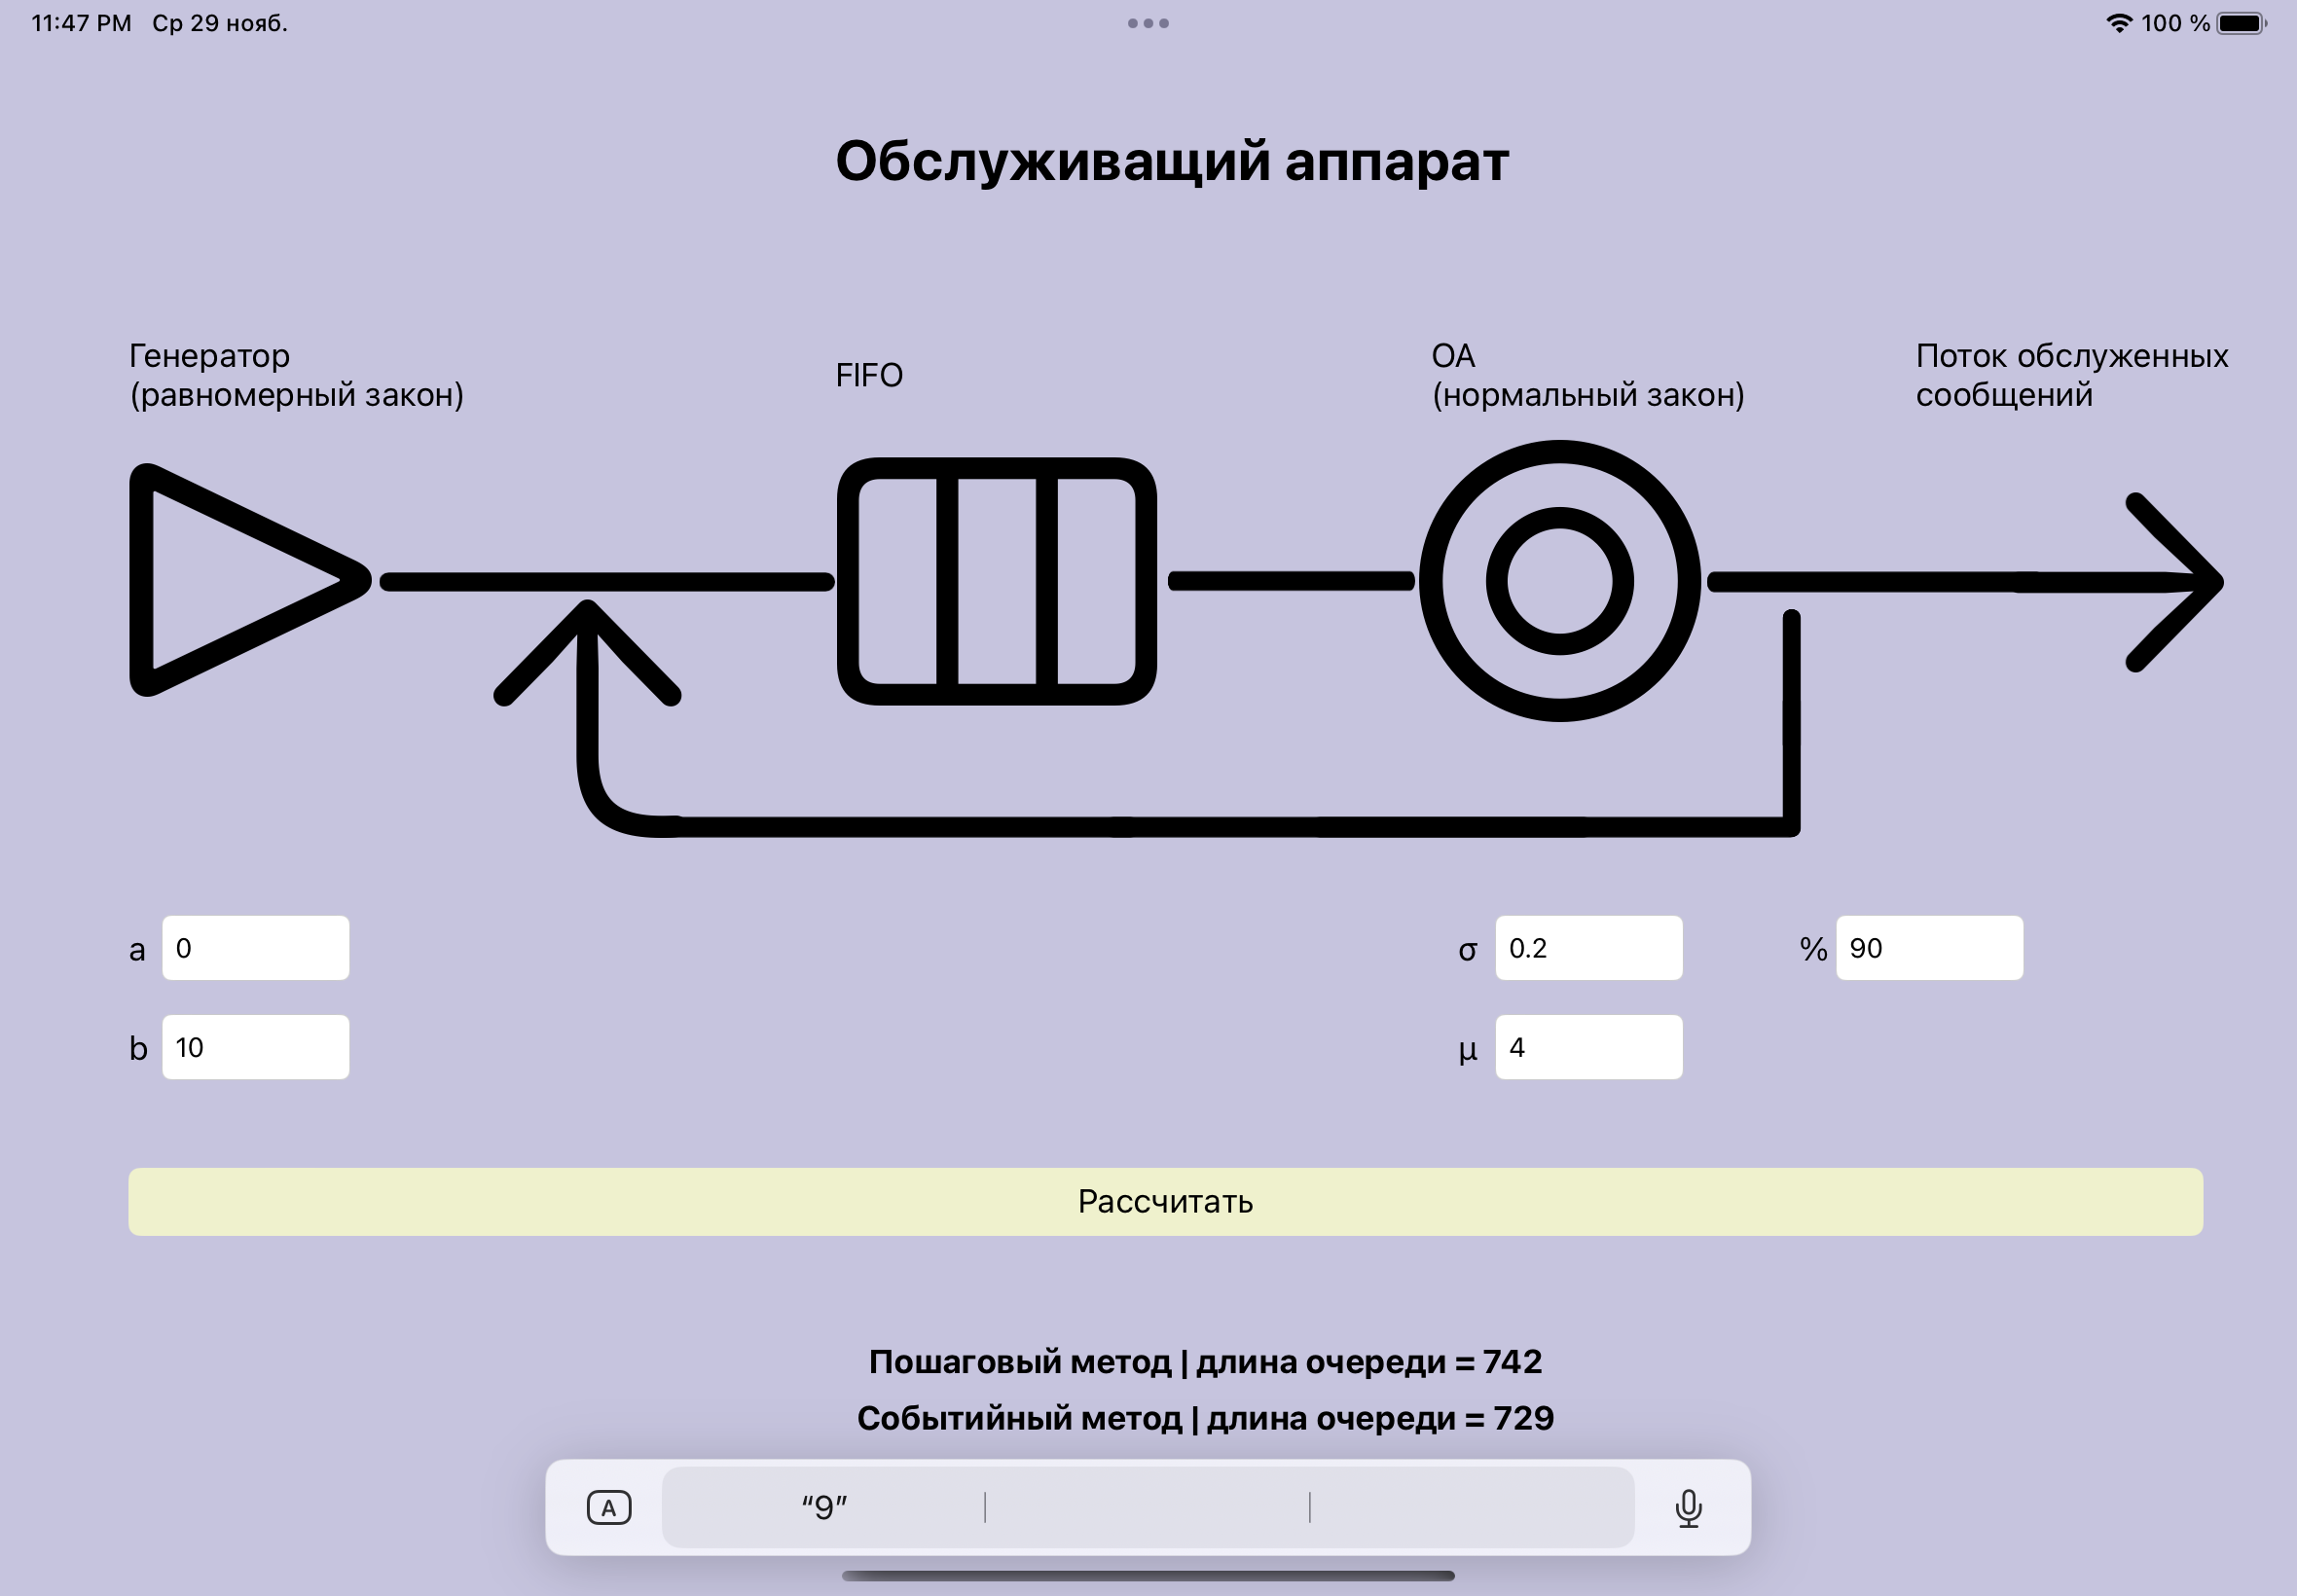
\includegraphics[scale = 0.15]{img/ex5.png}}
		\caption{Пример 5. Генератор и обслуживающий автомат работают с примерно одинаковой производительностью, но есть процент возврата  -- 90\%}
		\label{fig5:image}
	\end{center}
\end{figure}

\newpage

